\begin{frame}[fragile]

\frametitle{Git: Undoing changes}


\begin{onlyenv}<1>

Modified --\textgreater Unmodified:

\begin{lstlisting}[language=Bash]
git checkout -- path/to/file
\end{lstlisting}

\end{onlyenv}

\begin{onlyenv}<2>

Staged --\textgreater Modified:

\begin{lstlisting}[language=Bash]
git reset HEAD path/to/file
\end{lstlisting}

\end{onlyenv}

\begin{onlyenv}<3>

Commited --\textgreater Staged:

\begin{lstlisting}[language=Bash]
git reset [--mixed] HEAD~N
\end{lstlisting}

\end{onlyenv}

\begin{onlyenv}<4>

Already pushed:

\begin{lstlisting}[language=Bash]
git revert commit-sha
\end{lstlisting}

\end{onlyenv}


\begin{figure}
\centering
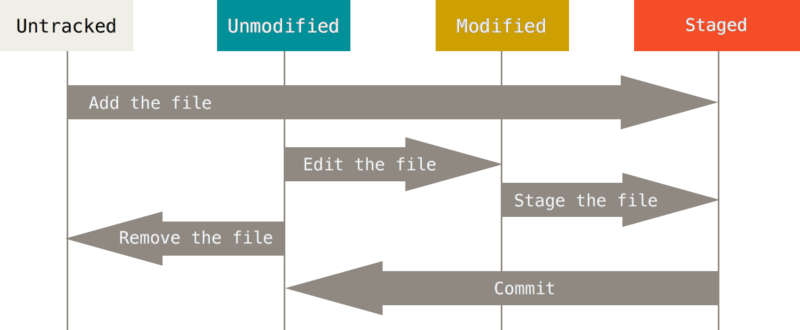
\includegraphics[scale=0.25]{git-lifecycle-file.png}
\caption{File lifecycle. From \href{https://git-scm.com/book/en/v2/Git-Basics-Recording-Changes-to-the-Repository}{Git SCM}}
\end{figure}

\end{frame}